\documentclass{FR16} 
\setlength{\parindent}{3em}
\setlength{\parskip}{1em}
\renewcommand{\baselinestretch}{1.5}
\begin{document}


\maketitle

\tableofcontents
\newpage

\section{Introducción}
El objetivo de este proyecto es crear un sistema para gestionar el funcionamiento del refugio de animales para servicios públicos o para empresas privadas. El trabajo propuesto se centra en el desarrollo de bases de datos, aplicación y documentación para ellos. El sistema es una aplicación Java que permite interactuar con la Base de datos Oracle.

Este aplicación permite llevar un registro de los animales ingresados, sus vacunas y procedimientos. También se mantiene un registro de las familias que toman el animal del refugio o lo devuelven.

Las herramientas de desarrollo fueron Oracle Database Express, el lenguaje pl/SQL para la creación de bases de datos y el lenguaje de programación Java.

\newpage

\section{Descripción del contexto y requisitos funcionales y no funcionales}
\subsection{Descripción del contexto}
\begin{center}
Descripción del contexto
\end{center}


\subsection{Requisitos funcionales y no funcionales}
\begin{center}
Requisitos funcionales
\end{center}

\newpage

\section{Diseño lógico y físico del sistema}
\subsection{Diagrama de clases}
\begin{figure}[H]
\centering
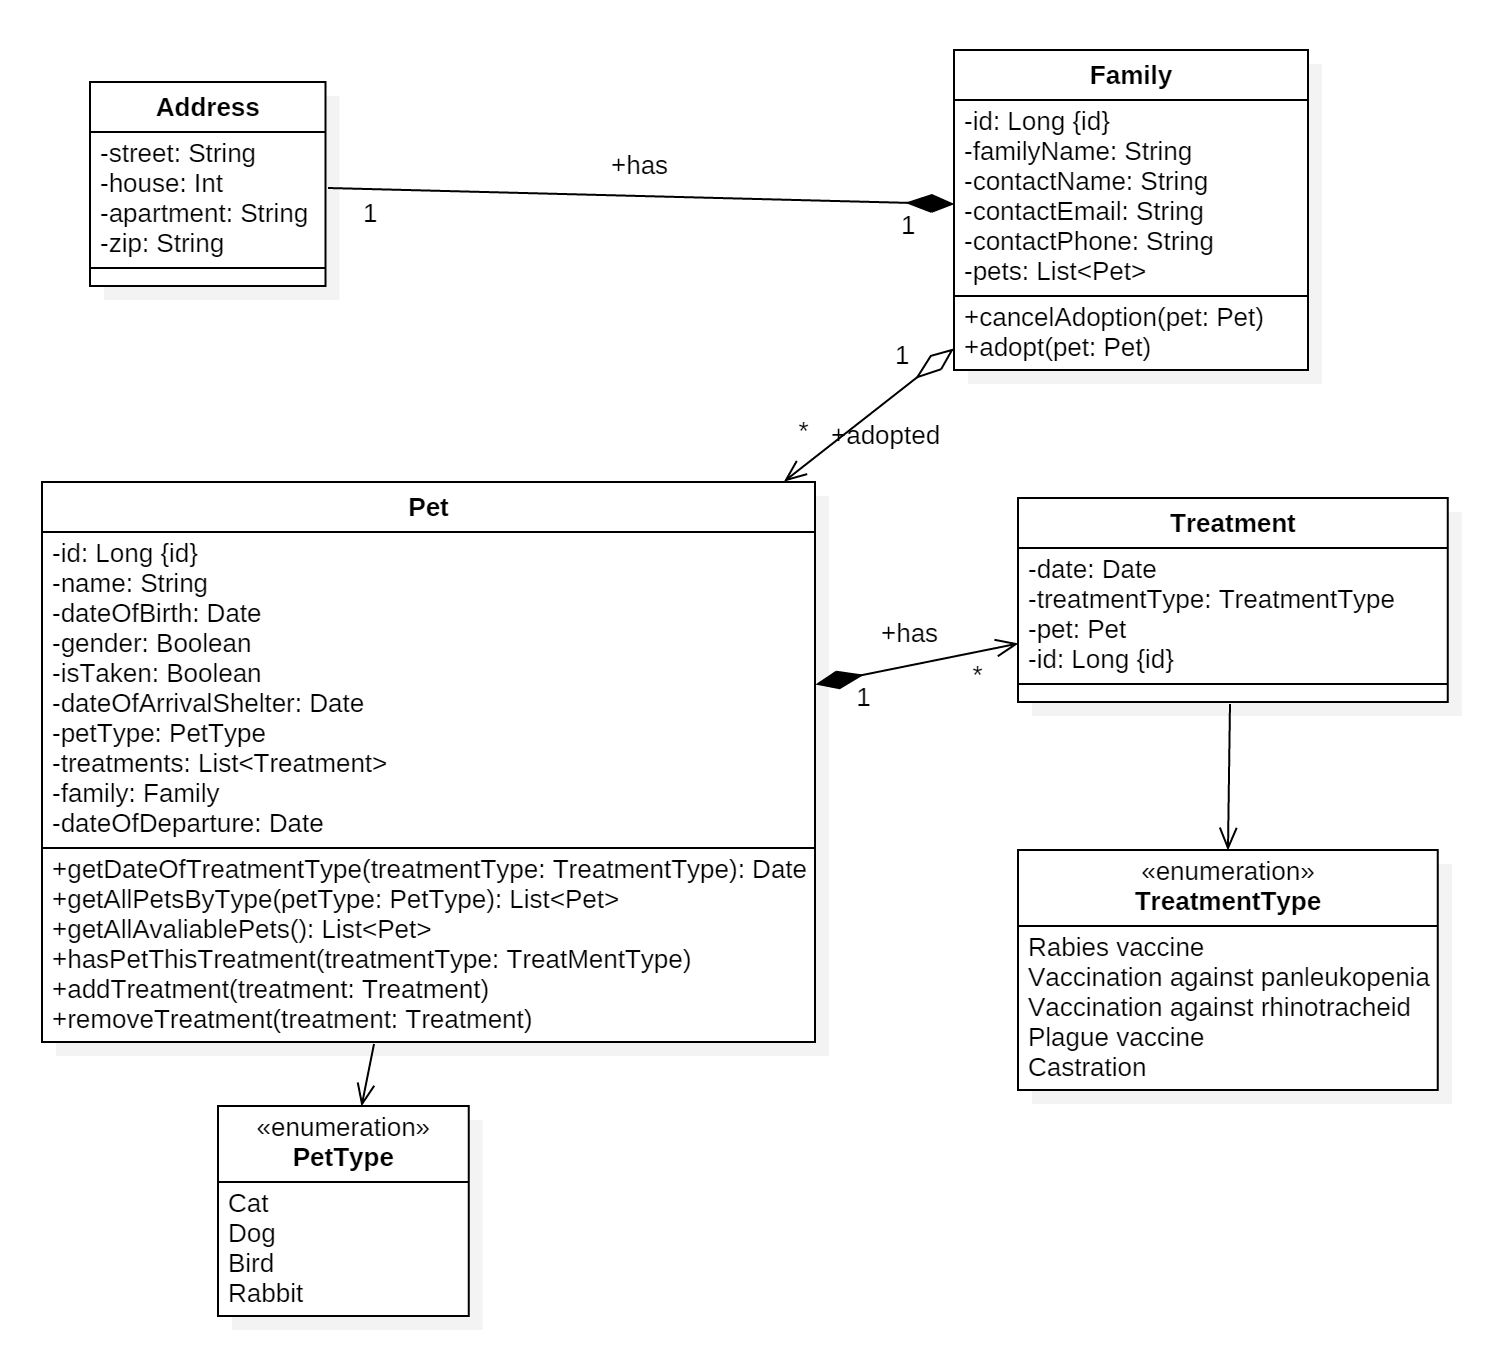
\includegraphics[width=1\textwidth]{Logical View.png}
\caption{\label{fig:1}Diagrama de clases.}
\end{figure}

\newpage

El \textbf{diagrama de clases} para esta aplicación consta de 4 clases y 2 enumeraciones. La tabla 'Pet' almacena toda la información relacionada con ella. La tabla está vinculada a la tabla 'Treatment' por la relación composición, que almacena todos los procedimientos en curso.Cada tipo de 'Treatment' tiene 'TreatmentType'. También hay una relación con la tabla 'Familia' agregación, ya que no todos en la tabla 'Pet'   tienen 'Family'. Cada mascota tiene un tipo que existe en la enumeración 'PetType'.

\subsection{Esquema lógico O / R específico}
\begin{center}
Esquema lógico O / R específico
\end{center}


\subsection{Diseño físico}
\begin{center}
Physical desing
\end{center}
\newpage

\section{Desarrollo del sistema}

\subsection{Tipos}

\begin{lstlisting}[language=Sql, basicstyle=\scriptsize]
create or replace type Address_objtyp  as object (
    street    varchar(500),
    house     number,
    apartment varchar(500),
    zip       varchar(500),
    MEMBER PROCEDURE display
    
);

/

create or replace type TreatmentType_objtyp  as object (
    id number,
    treatmentTypeTitle varchar(500)
);
/

create or replace type PetType_objtyp as object (
    petTypeTitle varchar(500),
    CONSTRUCTOR FUNCTION petType_objtyp( petTypeTitle varchar)
    RETURN SELF AS RESULT
);

-- forward declaration of Pet_objtyp
-- create or replace type Pet_objtyp;
/

create or replace type Treatment_objtyp  as object (
    id number,
    treatmentDate date,
    treatmentType varchar(500),
    MEMBER PROCEDURE display);


/

create or replace type TreatmentList_vartyp  as table of Treatment_objtyp;

/

create or replace type Family_objtyp  as object (
    id number,
    familyName varchar(500),
    contactName varchar(500),
    contactEmail varchar(500),
    contactPhone varchar(500),
    Address_obj Address_objtyp,
    MEMBER PROCEDURE display,
    MEMBER PROCEDURE setContactPhone(newPhone varchar),
    MEMBER PROCEDURE setEmail(newEmail varchar),
    MEMBER PROCEDURE setAddress(newAddress Address_objtyp),
    MEMBER PROCEDURE deleteFamily
    );

/

create or replace type FamilyList_vartyp as table of Family_objtyp;

/
create or replace type Pet_objtyp  as object (
    id number,
    name varchar(500),
    dateOfBirth date,
    gender NUMBER(1,0),
    isTaken NUMBER(1,0),
    dateOfArrivalShelter date,
    petType varchar(200),
    Treatments_List TreatmentList_vartyp,
    dateOfDeparture date,
    FamilyRef REF Family_objtyp,
    MEMBER FUNCTION hasPetThisTreatment(treatmentType varchar)    
    return number,
    MEMBER FUNCTION getALLTreatments                              
    return TreatmentList_vartyp,
    MEMBER PROCEDURE adoptByFamily(idFamily number),
    MEMBER PROCEDURE cancelAdoption,
    MEMBER PROCEDURE DISPLAY,
    MEMBER PROCEDURE addTreatment(treatmentType varchar, dateOfTr date),
    MEMBER PROCEDURE setDateOfDep(dateOfDep date),
    MEMBER PROCEDURE setName(newName1 varchar),
    MEMBER PROCEDURE setDateOfBirth(dateOfBirth date),
    MEMBER PROCEDURE setdateOfArrivalShelter(dateOfArrivalShelter date),
    MEMBER PROCEDURE setPetType(petTypepet varchar),
    MEMBER PROCEDURE deletePet
);

/

create or replace type PetsList_vartyp  as table of Pet_objtyp;

/
\end{lstlisting}
\newpage

\subsection{Tablas}
\begin{lstlisting}[language=Sql, basicstyle=\scriptsize]
drop table TreatmentType_objtab force;

drop table Pet_objtab force;

drop table Family_objtab force;


create table TreatmentType_objtab of TreatmentType_objtyp (id primary key) 
object identifier is primary key;

/

alter table TreatmentType_objtab
ADD CONSTRAINT unique_tr_type_title unique(treatmentTypeTitle);

/

create table Family_objtab of Family_objtyp (id primary key) 
object identifier is primary key;
/

alter table Family_objtab
ADD CONSTRAINT unique_fam_phone unique(contactPhone);
/

create table Pet_objtab of Pet_objtyp 
(primary key (id),
FOREIGN KEY (FamilyRef) REFERENCES Family_objtab)
object identifier is primary key 
nested table Treatments_List store as Pets_Treatments((
    PRIMARY KEY(NESTED_TABLE_ID, id))
    ORGANIZATION INDEX COMPRESS);
/


alter table  Pet_objtab 
ADD CONSTRAINT petType_notNull check ( petType is not null );
/

\end{lstlisting}
\newpage

\subsection{Secuencias}
\begin{lstlisting}[language=Sql, basicstyle=\scriptsize]
--sequence for treatmentType.id
CREATE SEQUENCE treatmentTypeTab_id_seq
    INCREMENT BY 1
    START WITH 1
    MAXVALUE 5000;
/

--sequence for treatmentType.id
CREATE SEQUENCE petTab_id_seq
    INCREMENT BY 1
    START WITH 1
    MAXVALUE 5000;
/

--sequence for treatments.id
CREATE SEQUENCE treatmentTab_id_seq
    INCREMENT BY 1
    START WITH 1
    MAXVALUE 5000;
/

--sequence for treatmentType.id
CREATE SEQUENCE familyTab_id_seq
    INCREMENT BY 1
    START WITH 1
    MAXVALUE 5000;
/
\end{lstlisting}
\newpage

\subsection{Disparadores}
\begin{lstlisting}[language=Sql, basicstyle=\scriptsize]
--trigger on treatmentType inserting
CREATE OR REPLACE TRIGGER treatmentType_on_insert
    BEFORE INSERT ON TreatmentType_objtab
    FOR EACH ROW
        BEGIN 
            SELECT treatmentTypeTab_id_seq.nextval
            INTO :new.id
            FROM dual;
        END;
/

--trigger on Pet_objtab inserting
CREATE OR REPLACE TRIGGER PetType_objtab_on_insert
    BEFORE INSERT ON  Pet_objtab
    FOR EACH ROW
        BEGIN 
            SELECT petTab_id_seq.nextval
            INTO :new.id
            FROM dual;
        END;
/        

--trigger on familyTab_id_seq inserting
CREATE OR REPLACE TRIGGER FamilyType_objtab_on_insert
    BEFORE INSERT ON Family_objtab
    FOR EACH ROW
        BEGIN 
            SELECT familyTab_id_seq.nextval
            INTO :new.id
            FROM dual;
        END;
/ 
\end{lstlisting}
\newpage

\subsection{Cuerpos de Tipos}
\begin{lstlisting}[language=Sql, basicstyle=\scriptsize]
--Pet type body
CREATE OR REPLACE TYPE BODY PetType_objtyp AS 
    CONSTRUCTOR FUNCTION petType_objtyp( petTypeTitle varchar)
        RETURN SELF AS RESULT IS
            BEGIN
                IF LOWER(TRIM(petTypeTitle)) IN ('dog', 'cat')
                    THEN 
                        SELF.petTypeTitle := LOWER(TRIM(petTypeTitle));
                ELSE
                    RAISE_APPLICATION_ERROR(-20999,'Unknown type "' 
                    || LOWER(TRIM(petTypeTitle)) || '"');
                END IF;
        RETURN;
    END;

END;
/

--Address type body--
CREATE OR REPLACE TYPE BODY Address_objtyp AS
    MEMBER PROCEDURE display IS
        BEGIN
            DBMS_OUTPUT.PUT_LINE ('address: street: ' || self.street || ', house: '||
            self.house || ', apartment: ' || self.apartment  ||
            ', zip: ' || self.zip) ;
        END;


END;
/

--Family type body--
CREATE OR REPLACE TYPE BODY Family_objtyp AS
    MEMBER PROCEDURE display IS
        BEGIN
            DBMS_OUTPUT.PUT_LINE ('id: ' || self.id || ', family name: '||
            self.familyName || ', contact name: ' || self.contactName ||
            ', email: ' || self.contactEmail || ', phone: ' || self.contactPhone);
            self.Address_obj.display;
        END;

    MEMBER PROCEDURE setContactPhone(newPhone varchar) IS
        BEGIN 
            UPDATE Family_objtab 
            SET contactPhone = newPhone
            WHERE id = SELF.id;
        END;

    MEMBER PROCEDURE setEmail(newEmail varchar) IS
        BEGIN 
            UPDATE Family_objtab 
            SET contactEmail = newEmail
            WHERE id = SELF.id;
        END;

    MEMBER PROCEDURE setAddress(newAddress Address_objtyp) IS
        BEGIN 
            UPDATE Family_objtab 
            SET Address_obj = newAddress
            WHERE id = SELF.id;
        END;  

    MEMBER PROCEDURE deleteFamily IS
        BEGIN 
            DELETE FROM Family_objtab 
            WHERE id = SELF.id;
        END;  
END;
         
/

CREATE OR REPLACE TYPE BODY Treatment_objtyp AS
    MEMBER PROCEDURE display IS
        BEGIN
            DBMS_OUTPUT.PUT_LINE ('id: ' || self.id || ', date: '||
            self.treatmentDate || ', type: ' || self.treatmentType);
            
        END;
END;        
/

CREATE OR REPLACE TYPE BODY Pet_objtyp AS 
--add treatment to the pet
    MEMBER PROCEDURE addTreatment(treatmentType varchar, dateOfTr date) IS
        treatmentType_title VARCHAR(200);
        NULL_TABLE EXCEPTION;
        PRAGMA EXCEPTION_INIT (NULL_TABLE, -22908);
    BEGIN
        BEGIN
            SELECT t.treatmentTypeTitle INTO 
            treatmentType_title 
            FROM TreatmentType_objtab t
            WHERE t.treatmentTypeTitle = treatmentType;
    
        EXCEPTION
             WHEN NO_DATA_FOUND THEN
                 raise_application_error (-20001, 'No such treatment ' 
                 || treatmentType ||' check treatments type with 
                 getAllTypeTreatments function');
    
        END;
        BEGIN
        INSERT INTO TABLE (
            SELECT p.Treatments_List
            FROM Pet_objtab p
            WHERE p.id = self.id
        )
        SELECT treatmentTab_id_seq.nextval, dateOfTr, t.treatmentTypeTitle
        FROM TreatmentType_objtab t
        WHERE t.treatmentTypeTitle = LOWER(treatmentType);

        EXCEPTION
                WHEN NULL_TABLE THEN
                UPDATE Pet_objtab SET Treatments_List = TreatmentList_vartyp()
                     WHERE id = self.id;
                INSERT INTO TABLE (
                    SELECT p.Treatments_List
                    FROM Pet_objtab p
                    WHERE p.id = self.id)
                SELECT treatmentTab_id_seq.nextval, dateOfTr, 
                    t.treatmentTypeTitle
                    FROM TreatmentType_objtab t
                    WHERE t.treatmentTypeTitle = LOWER(treatmentType);
        
        END;      
    END;
    MEMBER PROCEDURE DISPLAY IS
        BEGIN
            DBMS_OUTPUT.PUT_LINE('Pet: ' || self.id ||', name: ' || self.name ||
            ', type: ' || self.petType || ', gender:' 
            || self.gender || 'is taken?: ' || self.isTaken);
        END;


    MEMBER FUNCTION getALLTreatments return TreatmentList_vartyp IS
        BEGIN
            RETURN self.Treatments_List; 
        END;    

    MEMBER PROCEDURE cancelAdoption IS
    BEGIN
            UPDATE Pet_objtab 
            SET isTaken = 0,
                FamilyRef = NULL
            WHERE id = self.id;
    END;          

    MEMBER PROCEDURE adoptByFamily(idFamily number) IS
        familyRef_obj ref Family_objtyp;
        BEGIN
            SELECT REF (f) INTO familyRef_obj 
            FROM Family_objTab f
            WHERE id = idFamily;

            UPDATE Pet_objtab
            SET isTaken = 1,
                FamilyRef = familyRef_obj 
            WHERE id = self.id;

        END;   

     MEMBER FUNCTION hasPetThisTreatment(treatmentType varchar) return number IS
        countNum number;
        i INTEGER;
        BEGIN
            countNum := 0;
               FOR i in 1..SELF.Treatments_List.COUNT LOOP
               if(self.Treatments_List(i).treatmentType = LOWER(treatmentType)) then
                    countNum := countNum + 1;
                END IF;    
            END LOOP; 

            IF (countNum > 0) then
                RETURN 1;
            ELSE RETURN 0;
            END If;

        END; 

    MEMBER PROCEDURE setDateOfDep(dateOfDep date) IS
         BEGIN 
            UPDATE Pet_objtab 
            SET dateOfDeparture = dateOfDep
            WHERE id = SELF.id;
        END; 

    MEMBER PROCEDURE setName(newName1 varchar) IS
        BEGIN 
            UPDATE Pet_objtab
            SET name = newName1
            WHERE id = SELF.id;
        END; 

     MEMBER PROCEDURE setDateOfBirth(dateOfBirth date) IS
        BEGIN 
            UPDATE Pet_objtab 
            SET dateOfBirth = dateOfBirth
            WHERE id = SELF.id;
        END;

        MEMBER PROCEDURE setdateOfArrivalShelter(dateOfArrivalShelter date) IS
        BEGIN 
            UPDATE Pet_objtab 
            SET dateOfArrivalShelter = dateOfArrivalShelter
            WHERE id = SELF.id;
        END;

        MEMBER PROCEDURE setPetType(petTypepet varchar) IS
        BEGIN 
            UPDATE Pet_objtab 
            SET petType = petType_objtyp(petTypepet).petTypeTitle
            WHERE id = SELF.id;
        END; 

    MEMBER PROCEDURE deletePet IS 
        BEGIN
            DELETE FROM Pet_objtab 
            WHERE id = SELF.id;
        END;
         
END;

/
\end{lstlisting}
\newpage

\subsection{Paquete}
\begin{lstlisting}[language=Sql, basicstyle=\scriptsize]
CREATE OR REPLACE PACKAGE SHELTER AS

--TO-DO: to debug
    FUNCTION createAddress(street varchar, house number, 
    apartment varchar, zip varchar)      
    RETURN Address_objtyp;
    
     PROCEDURE createTreatmentType(treatmentTypeName varchar);

    FUNCTION getAllPetsByType(petType varchar)              
    RETURN PetsList_vartyp;
    FUNCTION getAllAvailablePets                            
    RETURN PetsList_vartyp;
    FUNCTION getPetById(id number)                          
    RETURN Pet_objtyp;
    FUNCTION hasPetThisTreatment(petId number, treatmentType varchar)
    RETURN number;
    FUNCTION getALLTreatments(petId number)                              
    RETURN TreatmentList_vartyp;
    PROCEDURE createPet(petName varchar, gender number, typeName varchar, 
    dateOfArrivalInShelter date);
    PROCEDURE addTreatmentToPet(petId number, treatmentName varchar);
    PROCEDURE deletePet(petId number); 
    PROCEDURE setPetType(petId number, petType varchar);
    PROCEDURE setPetName(petId number, newNamePet varchar);
    PROCEDURE setDateOfBirth(petId number, dateOfBirth date);
    PROCEDURE setdateOfArrivalShelter(petId number, dateOfArrivalShelter date);
    PROCEDURE adoptByFamily(petId number, idFamily number);
    PROCEDURE cancelAdoption(petId number);

    PROCEDURE createFamily(familyName varchar, contactName varchar, 
    contactPhone varchar, contactEmail varchar, famAdress Address_objtyp);
    PROCEDURE setFamilyEmail(familyId number, newEmail varchar);
    PROCEDURE setFamilyAddress(familyId number, newAddress Address_objtyp);
    PROCEDURE setFamilyPhone(familyId number, newPhone varchar);
    PROCEDURE deleteFamily(familyId number);
    FUNCTION getAllFamilies                                    
    RETURN FamilyList_vartyp;
    FUNCTION getFamilyById(id number)                         
    RETURN Family_objtyp;
    FUNCTION getFamilyByPhone(phone varchar)                  
    RETURN Family_objtyp;
    FUNCTION getFamilyIdByPhone(phone varchar)                 
    RETURN number;
    

END SHELTER;
/

CREATE OR REPLACE PACKAGE BODY SHELTER IS

--type's functions 
 PROCEDURE createTreatmentType(treatmentTypeName varchar) IS
    BEGIN 
        INSERT INTO TreatmentType_objtab
        (treatmentTypeTitle)
        VALUES
        (treatmentTypeName);
    END;

--address's functions
   FUNCTION createAddress(street varchar, house number, 
   apartment varchar, zip varchar) 
    RETURN Address_objtyp IS
    newAddress Address_objtyp;
        BEGIN
            newAddress := Address_objtyp(street, house, 
            apartment, zip);
            
            RETURN newAddress;
        END;

--pet's functions

    PROCEDURE createPet(petName varchar, gender number, typeName varchar,
    dateOfArrivalInShelter date) IS
        treatmentsList TreatmentList_vartyp := TreatmentList_vartyp();
        BEGIN
            INSERT INTO Pet_objtab
            (name, gender, isTaken, dateOfArrivalShelter, 
            petType, Treatments_List)
            VALUES
            (petName, gender, 0, dateOfArrivalInShelter, 
            petType_objtyp(typeName).petTypeTitle, treatmentsList);
        END;

    FUNCTION getAllPetsByType(petType varchar) return PetsList_vartyp IS
        pet Pet_objtyp;

        pets PetsList_vartyp := PetsList_vartyp();

        CURSOR allPetByType IS
		SELECT  *
		FROM Pet_objtab
        WHERE petType = petType_objtyp(petType).petTypeTitle;

        BEGIN 
		    FOR petRow IN allPetByType LOOP
                
                SELECT VALUE(p) INTO pet
                FROM Pet_objtab p
                WHERE id = petRow.id;

                 pets.extend();
                 pets(pets.count) := pet;
                 pet.display();

            END LOOP;

            RETURN pets;
        END;


    FUNCTION getAllAvailablePets return PetsList_vartyp IS
        pet Pet_objtyp;
        pets PetsList_vartyp := PetsList_vartyp();

        CURSOR allPetByType IS
		SELECT  *
		FROM Pet_objtab
        WHERE isTaken = 0;

        BEGIN 
		    FOR petRow IN allPetByType LOOP
                
                SELECT VALUE(p) INTO pet
                FROM Pet_objtab p
                WHERE id = petRow.id;

                 pets.extend();
                 pets(pets.count) := pet;
                 pet.display();

            END LOOP;

            RETURN pets;
        END;


    FUNCTION getPetById(id number)  RETURN Pet_objtyp IS
        pet Pet_objtyp;
        BEGIN
            BEGIN
            SELECT VALUE(p) INTO pet
                FROM Pet_objtab p
                WHERE p.id = id;

            EXCEPTION
             WHEN NO_DATA_FOUND THEN
                 raise_application_error (-20001, 'No such pet ');
            END;
            BEGIN
               RETURN pet;
            END; 
    END;


    PROCEDURE addTreatmentToPet(petId number, treatmentName varchar) IS
        pet Pet_objtyp;
        BEGIN
           pet := getPetById(petId);
           pet.addTreatment(treatmentName, sysdate);
        END; 

    PROCEDURE deletePet(petId number) IS
        pet Pet_objtyp;
        BEGIN
            pet := getPetById(petId);
            pet.deletePet();
        END;

    PROCEDURE adoptByFamily(petId number, idFamily number) IS
        pet Pet_objtyp;
        BEGIN
            pet := getPetById(petId);
            pet.adoptByFamily(idFamily); 
        END; 

    PROCEDURE cancelAdoption(petId number) IS
        pet Pet_objtyp;
        BEGIN
            pet := getPetById(petId);
            pet.cancelAdoption(); 
        END;

     PROCEDURE setPetType(petId number, petType varchar) IS
        pet Pet_objtyp;
        BEGIN
            pet := getPetById(petId);
            pet.setPetType(petType);
        END;    

    PROCEDURE setPetName(petId number, newNamePet varchar) IS
        pet Pet_objtyp;
        BEGIN
            pet := getPetById(petId);
            pet.setName(newNamePet);
        END;
    
    PROCEDURE setDateOfBirth(petId number, dateOfBirth date) IS
        pet Pet_objtyp;
        BEGIN
            pet := getPetById(petId);
            pet.setDateOfBirth(dateOfBirth);
        END; 

    PROCEDURE setdateOfArrivalShelter(petId number, dateOfArrivalShelter date) 
    IS
        pet Pet_objtyp;
        BEGIN
            pet := getPetById(petId);
            pet.setdateOfArrivalShelter(dateOfArrivalShelter);
        END; 

    FUNCTION hasPetThisTreatment(petId number, treatmentType varchar)    
    RETURN number IS
        pet Pet_objtyp;
        BEGIN 
            pet := getPetById(petId);
            RETURN pet.hasPetThisTreatment(treatmentType);
        END;  

    FUNCTION getALLTreatments(petId number)  RETURN TreatmentList_vartyp  
    IS
        pet Pet_objtyp;
        BEGIN 
            pet := getPetById(petId);
            RETURN pet.getALLTreatments;
        END;

--family's functions

PROCEDURE createFamily(familyName varchar, contactName varchar, 
contactPhone varchar, contactEmail varchar, famAdress Address_objtyp) 
IS
    BEGIN 
        INSERT INTO Family_objtab
        (familyName, contactName,contactEmail,contactPhone, Address_obj)
        VALUES
        (familyName, contactName,contactEmail, contactPhone, famAdress);
    END;

    FUNCTION getFamilyById(id number)  RETURN Family_objtyp IS
        family family_objtyp;
        BEGIN
            BEGIN
            SELECT VALUE(f) INTO family
                FROM Family_objtab f
                WHERE f.id = id;

            EXCEPTION
             WHEN NO_DATA_FOUND THEN
                 raise_application_error (-20001, 'No such family ');
            END;

            BEGIN
               RETURN family;
            END; 
    END;

    FUNCTION getFamilyByPhone(phone varchar)  RETURN Family_objtyp IS
        family family_objtyp;
        BEGIN
            BEGIN
            SELECT VALUE(f) INTO family
                FROM Family_objtab f
                WHERE f.contactPhone = phone;

            EXCEPTION
             WHEN NO_DATA_FOUND THEN
                 raise_application_error (-20001, 'No such family');
            END;

            BEGIN
               RETURN family;
            END; 
    END;

    FUNCTION getFamilyIdByPhone(phone varchar)  RETURN number IS
    family family_objtyp;
        BEGIN
            BEGIN
            SELECT VALUE(f) INTO family
                FROM Family_objtab f
                WHERE f.contactPhone = phone;

            EXCEPTION
             WHEN NO_DATA_FOUND THEN
                 raise_application_error (-20001, 'No such family');
            END;

            BEGIN
               RETURN family.id;
            END; 
    END;  

    FUNCTION getAllFamilies  return FamilyList_vartyp IS
        family Family_objtyp;
        families FamilyList_vartyp := FamilyList_vartyp();

        CURSOR allFamilies IS
		SELECT  *
		FROM Family_objtab;

        BEGIN 
		    FOR familyRow IN allFamilies LOOP
                
                SELECT VALUE(f) INTO family
                FROM Family_objtab f
                WHERE id = familyRow.id;

                 families.extend();
                 families(families.count) := family;
                 family.display();

            END LOOP;

            RETURN families;
        END;

    PROCEDURE deleteFamily(familyId number) IS
        family Family_objtyp;
        BEGIN
            family := getFamilyById(familyId);
            family.deleteFamily();
        END; 

    PROCEDURE setFamilyEmail(familyId number, newEmail varchar) IS
        family Family_objtyp;
        BEGIN
            family := getFamilyById(familyId);
            family.setEmail(newEmail);
        END; 

    PROCEDURE setFamilyAddress(familyId number, newAddress Address_objtyp) IS
        family Family_objtyp;
        BEGIN
            family := getFamilyById(familyId);
            family.setAddress(newAddress);
        END; 

    PROCEDURE setFamilyPhone(familyId number, newPhone varchar) IS
        family Family_objtyp;
        BEGIN
            family := getFamilyById(familyId);
            family.setContactPhone(newPhone);
        END; 
 

END;
/
\end{lstlisting}
\newpage

\subsection{Datos}
\begin{lstlisting}[language=Sql, basicstyle=\scriptsize]
INSERT ALL
INTO Family_objtab(familyName, contactName,contactEmail,contactPhone, Address_obj)
VALUES(
    'Sanches Garcia', 'Helena', 'helena_s@gmail.com', '662223554',
    Address_objtyp('Av. Ana de Viya', 1, '4A', '11010'))
INTO Family_objtab(familyName, contactName,contactEmail,contactPhone, Address_obj)
VALUES(
    'Gonzales Martinez', 'Maria Luisa', 'maria_l@gmail.com', '662778432',
    Address_objtyp('Av. Macroni', 32, '2B', '11011'))
INTO Family_objtab(familyName, contactName,contactEmail,contactPhone, Address_obj)
VALUES(
    'Ruiz Picasso', 'Pablo', 'pablo_p@gmail.com', '662990012',
    Address_objtyp('Av. Recreo', 14, '1A', '11008'))
INTO Family_objtab(familyName, contactName,contactEmail,contactPhone, Address_obj)
VALUES(
    'Perez Lopez', 'Rosario', 'rosario_p@gmail.com', '662888445',
    Address_objtyp('Av. de Peru', 3, '1A', '11007'))
INTO Family_objtab(familyName, contactName,contactEmail,contactPhone, Address_obj)
VALUES(
    'Martin Diaz', 'Teresa', 'teresa_m@gmail.com', '662334558',
    Address_objtyp('C. Santo Domingo', 16, '2С', '11006'))
 SELECT * FROM dual;

/

INSERT ALL
INTO TreatmentType_objtab VALUES('castration')
INTO TreatmentType_objtab VALUES('sterilization')
INTO TreatmentType_objtab VALUES('rabies')
INTO TreatmentType_objtab VALUES('rabies')
INTO TreatmentType_objtab VALUES('carnivores')
INTO TreatmentType_objtab VALUES('calvirus')
 SELECT * FROM dual;

/

INSERT ALL 
INTO Pet_objtab (name, dateOfBirth, gender, isTaken, dateOfArrivalShelter, petType,
Treatments_List, dateOfDeparture, FamilyRef REF)
     VALUES('Domingo', TO_DATE('01/01/2018', 'MM/DD/YYYY'), 1, 0, sysdate, 
     petType_objtyp('dog').petTypeTitle, TreatmentList_vartyp(), null, null)
INTO Pet_objtab (name, dateOfBirth, gender, isTaken, dateOfArrivalShelter, petType,
Treatments_List, dateOfDeparture, FamilyRef REF)
     VALUES('Kochi', TO_DATE('01/01/2017', 'MM/DD/YYYY'), 0, 0, sysdate, 
     petType_objtyp('cat').petTypeTitle, TreatmentList_vartyp(), null, null)
INTO Pet_objtab (name, dateOfBirth, gender, isTaken, dateOfArrivalShelter, petType,
Treatments_List, dateOfDeparture, FamilyRef REF)
     VALUES('Simba', TO_DATE('01/06/2018', 'MM/DD/YYYY'), 1, 0, sysdate, 
     petType_objtyp('cat').petTypeTitle, TreatmentList_vartyp(), null, null)
INTO Pet_objtab (name, dateOfBirth, gender, isTaken, dateOfArrivalShelter, petType,
Treatments_List, dateOfDeparture, FamilyRef REF)
     VALUES('Ringo', TO_DATE('01/06/2018', 'MM/DD/YYYY'), 1, 0, sysdate, 
     petType_objtyp('dog').petTypeTitle, TreatmentList_vartyp(), null, null)
INTO Pet_objtab (name, dateOfBirth, gender, isTaken, dateOfArrivalShelter, petType,
Treatments_List, dateOfDeparture, FamilyRef REF)
     VALUES('Kiko', TO_DATE('01/06/2019', 'MM/DD/YYYY'), 1, 0, sysdate, 
     petType_objtyp('dog').petTypeTitle, TreatmentList_vartyp(), null, null)
INTO Pet_objtab (name, dateOfBirth, gender, isTaken, dateOfArrivalShelter, petType,
Treatments_List, dateOfDeparture, FamilyRef REF)
     VALUES('Max', TO_DATE('01/01/2017', 'MM/DD/YYYY'), 1, 0, sysdate, 
     petType_objtyp('dog').petTypeTitle, TreatmentList_vartyp(), null, null)
INTO Pet_objtab (name, dateOfBirth, gender, isTaken, dateOfArrivalShelter, petType,
Treatments_List, dateOfDeparture, FamilyRef REF)
     VALUES('Kora', TO_DATE('01/06/2019', 'MM/DD/YYYY'), 0, 0, sysdate, 
     petType_objtyp('dog').petTypeTitle, TreatmentList_vartyp(), null, null)
INTO Pet_objtab (name, dateOfBirth, gender, isTaken, dateOfArrivalShelter, petType,
Treatments_List, dateOfDeparture, FamilyRef REF)
     VALUES('Greta', TO_DATE('01/01/2020', 'MM/DD/YYYY'), 0, 0, sysdate, 
     petType_objtyp('cat').petTypeTitle, TreatmentList_vartyp(), null, null)
SELECT * FROM dual;

/
\end{lstlisting}

\subsection{Lanzamiento}
\begin{lstlisting}[language=Sql, basicstyle=\scriptsize]
@types.sql;
/

@tables.sql;
/

@sequence.sql;
/

@triggers.sql;
/

@typebodies.sql;
/

@package.sql;
/

@test.sql;
/

\end{lstlisting}
\newpage


\section{Conclusiones}
\begin{center}
En este trabajo, se desarrolló el sistema de gestión del refugio de animales desde la perspectiva del gerente de la organización. El sistema permite mantener registros de animales, familias que recogen animales y servicios médicos para animales. El sistema consiste en una base de datos y una aplicación Java que proporciona acceso a la base y sus funciones.
\end{center}

\newpage
\begin{thebibliography}{9}

\bibitem{churchel}
Charchel, Clare, \emph{Beginning database desing}. APRESS, Second edition, 2007.

\bibitem{documentacion}
Database PL/SQL Language Reference, 

\hspace{10mm}\texttt{https://docs.oracle.com/cd/B28359_01/appdev.111/b28370/toc.htm}.

\bibitem{jdbc}
Java SE Technologies - Database, 

\hspace{10mm}\texttt{https://www.oracle.com/technetwork/java/javase/jdbc/index.html}.
\end{thebibliography}

\end{document}